\section{Simulation studies Paper V}
\begin{frame}
	\frametitle{Motivation}
	\begin{itemize}
		\item Test with a more detailed power plant model.
		\item Test with a more detailed power system model.
		\item Investigate some of the assumptions from previous papers.
	\end{itemize}
\end{frame}
\begin{frame}
	\frametitle{More detailed power plant model}
	\begin{figure}
		\includegraphics{./pictures/PID.tikz}
	\begin{figure}
		\includegraphics{./pictures/governor.tikz}
	\end{figure}
	\end{figure}
	\begin{figure}
		\includegraphics{./pictures/turbine.tikz}
	\end{figure}
\end{frame}
\begin{frame}
	\frametitle{More detailed power system model}
	\begin{columns}
		\begin{column}{0.5\textwidth}
			\begin{itemize}
				\item<1-> Added the frequency divider formula to the simple test system.
				\item<2-> Used the Nordic 44 test system in PSS/E.
			\end{itemize}
		\end{column}
		\begin{column}{0.5\textwidth}
			\begin{figure}
				\includegraphics<2>[width=\textwidth]{./pictures/Nordic44-Bilde}
			\end{figure}
			\begin{itemize}
					\item<1>[]
				\begin{equation}
					\omega_l = \mathbf{1}+\mathbf{D}(\omega_e-\mathbf{1})
				\end{equation}
				where
				\begin{equation}
					\mathbf{D} = -\mathbf{B}_{22}^{-1}\mathbf{B}_{21}
				\end{equation}
			\end{itemize}
		\end{column}
	\end{columns}
\end{frame}
\begin{frame}
	\frametitle{Identification cases}
	\begin{enumerate}
		\item \textbf{Case 1} Normal operation and speed feedback.
		\item \textbf{Case 2} Normal operation, speed feedback and PMU.
		\item \textbf{Case 3} Normal operation, frequency feedback and PMU.
		\item \textbf{Case 4} Open loop operation. 
	\end{enumerate}
	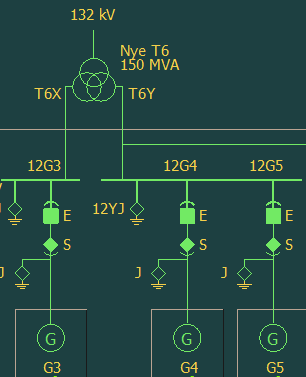
\includegraphics{./pictures/plant.tikz}
\end{frame}
\begin{frame}
	\frametitle{Test the different cases}
	\begin{figure}
		\includegraphics<1>[width=0.9\textwidth]{./pictures/G0_sim.tikz}
		\includegraphics<2>[width=0.9\textwidth]{./pictures/G_req_sim.tikz}
	\end{figure}
\end{frame}
\begin{frame}
	\frametitle{Test frequency assumption}
	\begin{figure}
		\includegraphics[width=0.9\textwidth]{./pictures/reactances.tikz}
	\end{figure}
\end{frame}
\begin{frame}
	\frametitle{Test backlash}
	\begin{figure}
		\includegraphics[width=0.9\textwidth]{./pictures/backlash.tikz}
	\end{figure}
\end{frame}
\begin{frame}
	\frametitle{Test deadband}
	\begin{figure}
		\includegraphics[width=0.9\textwidth]{./pictures/deadband.tikz}
	\end{figure}
\end{frame}
\begin{frame}
		\frametitle{Sensitivity function $S(s)$}
	\begin{figure}
		\includegraphics[width=0.9\textwidth]{./pictures/S_sim.tikz}
	\end{figure}
\end{frame}
\begin{frame}
		\frametitle{Disturbance rejection function $G_1(s)$}
	\begin{figure}
		\includegraphics[width=0.9\textwidth]{./pictures/G0_req_sim.tikz}
	\end{figure}
\end{frame}
\begin{frame}
	\frametitle{Comparison of stability margins}
			\begin{tabular}{c c c}
			\toprule
			Method & Median & Root mean square error (RMSE) \\
			$\max |S(j\Omega)|$ & $1.84$ & $0$ \\
			$\max |S(e^{j\Omega},\hat{\theta})|$, Case 1 & $1.84$ & $0.25$ \\
			$\max |S(e^{j\Omega},\hat{\theta})|$, Case 2 & $1.75$ & $0.34$ \\
			$\max |S(e^{j\Omega},\hat{\theta})|$, Case 3 & $1.74$ & $0.39$ \\
			$\max |S_{\min}(e^{j\Omega},\hat{\theta})|$ & $1.66$ & $0.25$ \\
			\bottomrule
	\end{tabular}
\end{frame}
\begin{frame}
	\frametitle{Comparison of estimated inertias}
	\begin{tabular}{c c c}
			\toprule
			Case & Median & RMSE \\
			Actual & $3.5$ & $0$ \\
			Case 1& $3.40$ & $0.46$ \\
			Case 2 & $3.33$ & $0.40$ \\
			Case 3 & $3.27$ & $0.43$ \\
			\bottomrule
	\end{tabular}
\end{frame}
\begin{frame}
	\frametitle{Major contributions}
	\begin{itemize}
		\item Tested the methods with a more detailed power plant model.
		\item Tested the methods  with a more detailed power system model.
		\item Investigate some of the assumptions from previous papers.
	\end{itemize}
\end{frame}

